%% ut-thesis.tex -- document template for graduate theses at UofT
%%
%% Copyright (c) 1998-2013 Francois Pitt <fpitt@cs.utoronto.ca>
%% last updated at 16:20 (EDT) on Wed 25 Sep 2013
%%
%% This work may be distributed and/or modified under the conditions of
%% the LaTeX Project Public License, either version 1.3c of this license
%% or (at your option) any later version.
%% The latest version of this license is in
%%     http://www.latex-project.org/lppl.txt
%% and version 1.3c or later is part of all distributions of LaTeX
%% version 2005/12/01 or later.
%%
%% This work has the LPPL maintenance status "maintained".
%%
%% The Current Maintainer of this work is
%% Francois Pitt <fpitt@cs.utoronto.ca>.
%%
%% This work consists of the files listed in the accompanying README.

%% SUMMARY OF FEATURES:
%%
%% All environments, commands, and options provided by the `ut-thesis'
%% class will be described below, at the point where they should appear
%% in the document.  See the file `ut-thesis.cls' for more details.
%%
%% To explicitly set the pagestyle of any blank page inserted with
%% \cleardoublepage, use one of \clearemptydoublepage,
%% \clearplaindoublepage, \clearthesisdoublepage, or
%% \clearstandarddoublepage (to use the style currently in effect).
%%
%% For single-spaced quotes or quotations, use the `longquote' and
%% `longquotation' environments.

%%%%%%%%%%%%         PREAMBLE         %%%%%%%%%%%%

%%  - Default settings format a final copy (single-sided, normal
%%    margins, one-and-a-half-spaced with single-spaced notes).
%%  - For a rough copy (double-sided, normal margins, double-spaced,
%%    with the word "DRAFT" printed at each corner of every page), use
%%    the `draft' option.
%%  - The default global line spacing can be changed with one of the
%%    options `singlespaced', `onehalfspaced', or `doublespaced'.
%%  - Footnotes and marginal notes are all single-spaced by default, but
%%    can be made to have the same spacing as the rest of the document
%%    by using the option `standardspacednotes'.
%%  - The size of the margins can be changed with one of the options:
%%     . `narrowmargins' (1 1/4" left, 3/4" others),
%%     . `normalmargins' (1 1/4" left, 1" others),
%%     . `widemargins' (1 1/4" all),
%%     . `extrawidemargins' (1 1/2" all).
%%  - The pagestyle of "cleared" pages (empty pages inserted in
%%    two-sided documents to put the next page on the right-hand side)
%%    can be set with one of the options `cleardoublepagestyleempty',
%%    `cleardoublepagestyleplain', or `cleardoublepagestylestandard'.
%%  - Any other standard option for the `report' document class can be
%%    used to override the default or draft settings (such as `10pt',
%%    `11pt', `12pt'), and standard LaTeX packages can be used to
%%    further customize the layout and/or formatting of the document.

%% *** Add any desired options. ***
\documentclass{ut-thesis}

%% *** Add \usepackage declarations here. ***
%% The standard packages `geometry' and `setspace' are already loaded by
%% `ut-thesis' -- see their documentation for details of the features
%% they provide.  In particular, you may use the \geometry command here
%% to adjust the margins if none of the ut-thesis options are suitable
%% (see the `geometry' package for details).  You may also use the
%% \setstretch command to set the line spacing to a value other than
%% single, one-and-a-half, or double spaced (see the `setspace' package
%% for details).

\usepackage{graphicx, float, booktabs, makecell, tikz, longtable, amsmath, bm}
\usetikzlibrary{calc}

%%%%%%%%%%%%%%%%%%%%%%%%%%%%%%%%%%%%%%%%%%%%%%%%%%%%%%%%%%%%%%%%%%%%%%%%
%%                                                                    %%
%%                   ***   I M P O R T A N T   ***                    %%
%%                                                                    %%
%%  Fill in the following fields with the required information:       %%
%%   - \degree{...}       name of the degree obtained                 %%
%%   - \department{...}   name of the graduate department             %%
%%   - \gradyear{...}     year of graduation                          %%
%%   - \author{...}       name of the author                          %%
%%   - \title{...}        title of the thesis                         %%
%%%%%%%%%%%%%%%%%%%%%%%%%%%%%%%%%%%%%%%%%%%%%%%%%%%%%%%%%%%%%%%%%%%%%%%%

%% *** Change this example to appropriate values. ***
\degree{Doctor of Philosophy}
\department{Civil Engineering}
\gradyear{2021}
\author{Jason Fraser Hawkins}
\title{Modelling Choice and Transition in a Market of Emerging Mobility Alternatives: Development of Econometric Foundations and Application in Greater Toronto Area}

%% *** NOTE ***
%% Put here all other formatting commands that belong in the preamble.
%% In particular, you should put all of your \newcommand's,
%% \newenvironment's, \newtheorem's, etc. (in other words, all the
%% global definitions that you will need throughout your thesis) in a
%% separate file and use "\input{filename}" to input it here.


%% *** Adjust the following settings as desired. ***

%% List only down to subsections in the table of contents;
%% 0=chapter, 1=section, 2=subsection, 3=subsubsection, etc.
\setcounter{tocdepth}{2}

%% Make each page fill up the entire page.
\flushbottom


%%%%%%%%%%%%      MAIN  DOCUMENT      %%%%%%%%%%%%

\begin{document}

%% This sets the page style and numbering for preliminary sections.
\begin{preliminary}

%% This generates the title page from the information given above.
\maketitle

%% There should be NOTHING between the title page and abstract.
%% However, if your document is two-sided and you want the abstract
%% _not_ to appear on the back of the title page, then uncomment the
%% following line.
%\cleardoublepage

%% This generates the abstract page, with the line spacing adjusted
%% according to SGS guidelines.
\begin{abstract}
%% *** Put your Abstract here. ***
%% (At most 150 words for M.Sc. or 350 words for Ph.D.)
\end{abstract}

%% Anything placed between the abstract and table of contents will
%% appear on a separate page since the abstract ends with \newpage and
%% the table of contents starts with \clearpage.  Use \cleardoublepage
%% for anything that you want to appear on a right-hand page.

%% This generates a "dedication" section, if needed -- just a paragraph
%% formatted flush right (uncomment to have it appear in the document).
%\begin{dedication}
%% *** Put your Dedication here. ***
%\end{dedication}

%% The `dedication' and `acknowledgements' sections do not create new
%% pages so if you want the two sections to appear on separate pages,
%% uncomment the following line.
%\newpage  % separate pages for dedication and acknowledgements

%% Alternatively, if you leave both on the same page, it is probably a
%% good idea to add a bit of extra vertical space in between the two --
%% for example, as follows (adjust as desired).
%\vspace{.5in}  % vertical space between dedication and acknowledgements

%% This generates an "acknowledgements" section, if needed
%% (uncomment to have it appear in the document).
%\begin{acknowledgements}
%% *** Put your Acknowledgements here. ***
%\end{acknowledgements}

%% This generates the Table of Contents (on a separate page).
\tableofcontents

%% This generates the List of Tables (on a separate page), if needed
%% (uncomment to have it appear in the document).
%\listoftables

%% This generates the List of Figures (on a separate page), if needed
%% (uncomment to have it appear in the document).
%\listoffigures

%% You can add commands here to generate any other material that belongs
%% in the head matter (for example, List of Plates, Index of Symbols, or
%% List of Appendices).

%% End of the preliminary sections: reset page style and numbering.
\end{preliminary}


%%%%%%%%%%%%%%%%%%%%%%%%%%%%%%%%%%%%%%%%%%%%%%%%%%%%%%%%%%%%%%%%%%%%%%%%
%%  Put your Chapters here; the easiest way to do this is to keep     %%
%%  each chapter in a separate file and `\include' all the files.     %%
%%  Each chapter file should start with "\chapter{ChapterName}".      %%
%%  Note that using `\include' instead of `\input' will make each     %%
%%  chapter start on a new page, and allow you to format only parts   %%
%%  of your thesis at a time by using `\includeonly'.                 %%
%%%%%%%%%%%%%%%%%%%%%%%%%%%%%%%%%%%%%%%%%%%%%%%%%%%%%%%%%%%%%%%%%%%%%%%%

%% *** Include chapter files here. ***
\chapter{Introduction}

\chapter{Literature Review}
\section{Integrated Land Use and Transportation Models}
Mostly pull from review paper and add at end.

\section{Residential Location Choice Models}
Draw from publications as we go along. I know the field fairly well. Ellickson and Lerman to Martinez to recent work in field and challenges in terms of endogeneity.

\section{Household Production}
Household production denotes a distinction in the economic literature between goods and services produced in the market and those produced in the home. Initial development of the model is attributed to Gary Becker and Jack Mincer in the 1960s \cite{Becker1965}. In his 1965 article, Becker outlines the lack of consideration given in the economics literature for the time allocation by households outside working hours. He references a decline in working hours and a dearth of attention for the role of non-compensated work. The classical economic philosophy is to consider consumers to trade productive work time for non-productive leisure time. Becker proposes a model structured about this metric of time to draw out the components of this, so called, leisure time. The theory is best summarized through a series of exemplar comparisons. Consider a household consisting of two adults and two children, who must consider the care of the children during the working day. The first option would be to send the children to daycare, in which case both parents would most likely need to work in order to pay the daycare fee. The second option would be for one parent to stay home and care for the children. This would save on daycare costs, and other household maintenance costs, but lead to a reduced monetary budget. The trade-off in household production theory is generally between 1) additional engagement in the market economy to increase the household budget and 2) devoting household time to the uncompensated production of the good or service. A second example would the production of food for consumption by the household. In general, the time required to produce food decreases with increasing monetary cost, such that a household will trade-off producing food from scratch and consuming a processed meal (whether at home or in a restaurant). Household production of food requires uncompensated time, while processed food requires additional monetary outlays - therefore additional income from compensated work. Becker proposes an adjustment of the classical consumption theory to include a time constraint, in addition to the traditional income constraint. His model was improved upon by Gronau \cite{Gronau1977} and DeSerpa \cite{DeSerpa1971}

%The income constraint can be written in terms of time as follows
% \begin{equation}
% 	T_w \bar{w} + m \leq M ,
% \end{equation}
% where $T_w$ is the number of working hours, $\bar{w}$ the wage rate, $m$ a measure of other income, and $M$ the total household income. An additional time constraint can be defined as follows
% \begin{equation}
% 	T_w + \sum_i^P T_i \leq T ,
% \end{equation}
% where $T_i$ is a vector of time spent at various household production activities and $T$ is the time budget (i.e. 24 hours in the day).

This theory has important implications for transportation and land use behaviour model theory. Transportation demand models that follow the activity based (ABM) or microsimulation paradigms are at their core models of time allocation. The time-space prism of Hagerstrand is a common method for structuring this class of transportation demand models \cite{Hagerstrand1970WhatScience}. It has a fairly intuitive interpretation given by constraints on available time (i.e. 24 hours in a day) and skeletal activities (i.e. work, school, and sleep) restricting the time available in which to conduct other activities. The spatial dimension enters as the time required to move between activities, with the time available for an activity being diminished by longer (therefore more time-consuming) travel. Habib has developed an activity scheduling model, based in random utility maximizing, that applies this theory of time expenditure. His CUSTOM framework iteratively develops the set of trips made by a person each day by referencing each destination choice against the available remaining time in the day and the decision to return home. A continuous time horizon is used in CUSTOM to fully capture the decision-making process. The model is fully based in econometric theory and empirical data, in contrast to the hard-wired rules of previous models.

Household production theory takes this principle a step further by incorporating the time constraint into the representation of the economy. Land use models has generally existed at the boundary between economic and transportation modelling. Its inclusion of residential and work location necessary means that land use modelling requires a representation of the cost of housing, the location of work opportunities, and the potential wage at each location. From the perspective of the transportation system, land use determines the length and distribution of trips (as well as mode of travel to a large extent). The focus of this thesis is how the links between these systems are represented in ILUT models. The traditional connection between land use and the economy is to spatially place economic activities within the model region. As discussed above, the connection between land use and transportation is through a measures of accessibility, generally measured as the logsum of a mode choice model or the number of opportunities (i.e. work and shopping) in close proximity. I propose time as the connection between all three systems. It is the organizing principle in activity scheduling and is a major contributor to residential location through the travel time to work and other opportunities. By adopting a form of household production theory, the time allocation of the household can be explicitly represented in economic models of the region.

Travel is negative space of activity participation

Focus on the math...

Becker to DeSerpa to Jara-Diaz

Beginning from Becker, the traditional model of household utility is of the form \cite{Becker1965}
\begin{equation}
	U = U(y_1,y_2,...,y_n),
\end{equation}
which is subject to the resource constraint \cite{Becker1965}
\begin{equation}
	\sum p_i y_i = I = W + V,
\end{equation}
where $y_i$ are market goods, $p_i$ are their prices, $I$ is the monetary income of the household, and $W$ and $V$ are the wage and other income components of the household income.

Becker starts from the statement that households "will be assumed to combine time and market goods to produce more basic commodities that directly enter their utility function" \cite[p. 495]{Becker1965}. These commodities are defined by
\begin{equation}
	Z_i = f_i(x_i, T_i),
\end{equation}
where $f_i$ is the definition of the household production function, $x_i$ are goods purchased on the market, and $T_i$ is time spent in the production of commodity $Z_i$. He then defines a utility function in terms of these new commodities
\begin{equation}
	U = U(Z_1,...Z_m) = U(x_1,...x_m; T_1,...T_m)
\end{equation}
and the new budget constraint defined by
\begin{equation}
	g(Z_1,...Z_m) = Z.
\end{equation}
He develops individual constraints for goods and time consumption, which are subsequently combined based on an assumption that time can be converted for goods by spending more time on paid work. This produces a single constrained
\begin{equation}
	\sum(p_i b_i + t_i \bar{w})Z_i = V + T \bar{w}
\end{equation}
with
\begin{equation}
	\pi_i = p_i b_i + t_i \bar{w}
\end{equation}
\begin{equation}
	S' = V + T \bar{w}.
\end{equation}
In this formulation, $b_i$ is the price of each good per unit of $Z_i$, $t_i$ is the input of time for each good per unit of $Z_i$, $\pi$ is the expenditure on each good, and $S'$ is the money income. This income is reduced either directly, through the purchase of goods given by $\sum p_i b_i Z_i$, or indirectly through the forfeiture of income, $\sum t_i \bar{w} Z_i$, by the use of time in consumption rather than work.

DeSerpa begins with a critique of Becker, who assumes that all time is uniformly priced at the average wage rate $\bar{w}$. He further extends the theory premised on a minimum time requirement in order to produce a commodity, which may be extended by the household if it obtains an additional utility by continued consumption of time engaged in the activity (i.e. consumption of the commodity). By removing the time prices from his model, DeSerpa maintains the set of two constraints (i.e. goods consumption and time consumption are independent). He defines an inequality constraint as follows
\begin{equation}
	T_i \geq a_i X_i,
\end{equation}
which states that time spent on the consumption of a good must be at least the minimum set of technological and institutional constraints. A major contribution of his work is this inequality, which he distinguishes as a \emph{time consumption constraint} and distinguishes from the \emph{time resource constraint} defining a maximum available time in the day. He gives the examples of a round of golf, movies, meals, road congestion, and reading as technology constraints. Institutional constraints would be speed limits, rigid work schedules, or banquets.

Another key component of the model is its distinction between \emph{value of time} and \emph{value of saving time}. Value of time as a resource has little meaning because it is not possible to extend time beyond the fixed 24 hours of the day. Value arises from time savings, which can be transferred to alternative higher utility usage. This value is defined by
\begin{equation}
	X_i = \frac{\mu}{\lambda} - \frac{U_{n+i}}{\lambda} = \frac{K_i}{\lambda}.
\end{equation}
This can be thought of as the marginal rate of substitution between time and money for allocation of time to consumption of $X_i$. In this equation, $\lambda$ is the shadow price of goods consumption and $\mu$ is the shadow price of time consumption from the maximization equation.

Jara-Diaz has extended this work in recent years (since about 2003). His model is defined by
\begin{equation}
	\max U = \Omega T_w^{\theta_w} \prod_i T_i^{\theta_i} \prod_j X_j^{\eta_j}
\end{equation}
\begin{equation}
	I + wT_w - \sum_j p_j X_j \geq 0 (giving \lambda)
\end{equation}
\begin{equation}
	\tau - T_w - \sum_i T_i = 0 (giving \mu)
\end{equation}
\begin{equation}
	T_i \geq f_i(X) \forall i (giving \kappa_i)
\end{equation}
\begin{equation}
	X_j \geq g_j(T) \forall j (giving \rho_j) .
\end{equation}
The utility is defined as Cobb-Douglas and Jara-Diaz connects the time and goods consumption through a technological relation.


\chapter{Conceptual Framework}
\section{Econometric Model Structure}
\subsection{Time and Goods Consumption}
The multiple discrete continuous extreme value (MDCEV) model of Bhat \cite{Bhat2005, Bhat2008TheExtensions} is used as a baseline model formulation. The utility function takes the form of a generalised variant of the translated CES utility function
\begin{equation}
    U(\textbf{x}) = \sum_{k=1}^K \frac{\gamma_k}{\alpha_k}\psi_k \left[\left(\frac{x_k}{\gamma_k}+1\right)^{\alpha_k} - 1\right]
\end{equation}

This takes the form of a linear expenditure system (LES) when $\alpha_k -> 0 \forall k$
\begin{equation}
    U(\textbf{x}) = \sum_{k=1}^K \gamma_k \psi_k \ln \left(\frac{x_k}{\gamma_k}+1\right) .
\end{equation}

Bhat formulates the MDCEV model as a direct utility function, which is constrained by a budget constraint on total consumption. This can take the form of a time constraint in the case of time-use models or a monetary constraint, as a function of income, in the case of expenditure models. In order to apply the household production function of DeSerpa \cite{DeSerpa1971}, the model must be constrained in both time and money. Castro et al. \cite{Castro2012AccommodatingModel} provides a system of multiple constraints and discuss identification issues with this extension to the MDCEV model structure. A separate set of constraints are also required, in the form of minimum time and money consumption constraints. These are the technology constraints defined by DeSerpa in his original formulation of household production \cite{DeSerpa1971}. Van Nostrand et al. \cite{VanNostrand2013AnalysisFramework} address this component of the model formulation in the context of long-distance vacation travel demand. The resulting MDCEV utility function takes the following form
\begin{equation}
    U(\textbf{x}) = \sum_{k=1}^K \gamma_k \psi_k \ln \left(\frac{x_k - x_k^\circ}{\gamma_k}+1\right)
\end{equation}

Astroza et al. \cite{Astroza2017AConsumption} present a first attempt at incorporating the DeSerpa household production function into the MDCEV model framework. An optimisation function can be defined for individuals $q$ ($q$ = 1,2,....Q), consuming goods $x_k$ ($k$=1,2,...K), allocating time $t_n$ to non-work activities ($n$=1,2,...N), and allocating time $t_w$ to the work activity. It takes the form

\begin{equation}\label{eq:util1}
    \max(U_q(\bm{x}_q,\bm{t}_q,\bm{t}_{qw})) = \sum_{k=1}^K u_k(x_{qk}) + \sum_{n=1}^N\widetilde{u}_n(t_{nq}) + \widetilde{u}_w(t_{wq})
\end{equation}

subject to the following constraints
\begin{subequations}\label{eq:st}
    \begin{align}
        &\sum_{k=1}^K p_{qk}x_{qk} = E_q + \omega_q t_{qw} \\
        &\sum_{n=1}^N t_{qn} + t_{qw} = T_q
    \end{align}
\end{subequations}

The value of time appears in both the money and time budget constraints, which adds an additional level of complex compared with the standard MDCEV model because it represents a multidimensional constraint. Fortunately, this complication can be isolated to the determination of $t_w$ and the other decision variables (i.e. $t_{qn}$ and $x_{qk}$) can be determined in the usual way. Taking account for minimum required consumption and time allocation, Norstrand et al. \cite{VanNostrand2013AnalysisFramework} provide the following utility function definitions
\begin{subequations}\label{eq:util2}
\begin{align}
    &u_k(x_{qk}) = 
    \begin{cases}
    \psi_{qk}x_{qk} & \text{if } x_{qk} \leq x_{qk}^\circ \\
    \psi_{qk}x_{qk}^\circ + \gamma_k \psi_k \ln \left(\frac{x_{qk} - x_{qk}^\circ}{\gamma_k}+1\right) & \text{otherwise}
    \end{cases} \\
    &\widetilde{u}_n(t_{qn}) = 
    \begin{cases}
    \psi_{qn}t_{qn} & \text{if } t_{qn} \leq t_{qn}^\circ \\
    \psi_{qn}t_{qn}^\circ + \gamma_n \psi_n \ln \left(\frac{t_{qn} - t_{qn}^\circ}{\gamma_n}+1\right) & \text{otherwise}
    \end{cases} \\
    &\widetilde{u}_w(t_{qw}) = 
    \begin{cases}
    \psi_{qw}t_{qw} & \text{if } t_{qw} \leq t_{qw}^\circ \\
    \psi_{qw}t_{qw}^\circ + \gamma_n \psi_n \ln \left(\frac{t_{qw} - t_{qw}^\circ}{\gamma_w}+1\right) & \text{otherwise}
    \end{cases}
\end{align}
\end{subequations}

The Lagrangian function for individual $q$ is defined by
\begin{equation}
    \mathcal{L}_q = U_q\left(\bm{x}_q,\bm{t}_q,\bm{t}_{qw}\right) + \lambda_q\left(E_q + \omega_q t_{qw} - \sum_{k=1}^K p_{qk}x_{qk}\right) + \mu_{q}\left(T_q - t_{qw} - \sum_{n=1}^N t_{qn}\right)
\end{equation}
where $\lambda_q$ and $\mu_q$ are multipliers for the time and money constraints, representing the marginal utilities of time and expenditure. The KKT first-order conditions are defined by
\begin{subequations}\label{eq:kkt1}
    \begin{align}
        &u_k'\left(x_{qk}^*\right) - \lambda_q p_{qk} = 0 & \text{if } x_{qk}^* > 0,k=1,2,...K \\
        &u_k'\left(x_{qk}^*\right) - \lambda_q p_{qk} < 0 & \text{if } x_{qk}^* = 0,k=1,2,...K \\
        &\widetilde{u}_n'\left(t_{qn}^*\right) - \mu_q = 0 & \text{if } t_{qn}^* > 0,n=1,2,...N \\
        &\widetilde{u}_n'\left(t_{qn}^*\right) - \mu_q < 0 & \text{if } t_{qn}^* = 0,n=1,2,...N \\
        &\widetilde{u}_w'\left(t_{qw}^*\right) +\omega_q \lambda_q - \mu_q = 0 & \text{if } t_{qw}^* > 0,w=1,2,...W \\
        &\widetilde{u}_w'\left(t_{qw}^*\right) +\omega_q \lambda_q - \mu_q < 0 & \text{if } t_{qw}^* = 0,w=1,2,...W
    \end{align}
\end{subequations}
where $u_{qk}'$, $\widetilde{u}_{qn}'$, and $\widetilde{u}_{qw}'$ are the marginal utility functions defined by
\begin{subequations}\label{eq:kkt2}
    \begin{align}
        &u_k'(x_{qk}^*) = 
        \begin{cases}
        \psi_{qk} & \text{if } x_{qk}^* \leq x_{qk}^\circ \\
        \psi_{qk}\left(\frac{x_{qk}^* - x_{qk}^\circ}{\gamma_k}+1\right)^{-1} & \text{otherwise}
        \end{cases} \\
        &\widetilde{u}_n'(t_{qn}^*) = 
        \begin{cases}
        \psi_{qn} & \text{if } t_{qn}^* \leq t_{qn}^\circ \\
        \psi_{qn} \left(\frac{t_{qn}^* - t_{qn}^\circ}{\gamma_n}+1\right)^{-1} & \text{otherwise}
        \end{cases} \\
        &\widetilde{u}_w'(t_{qw}^*) = 
        \begin{cases}
        \psi_{qw} & \text{if } t_{qw}^* \leq t_{qw}^\circ \\
        \psi_{qw} \left(\frac{t_{qw}^* - t_{qw}^\circ}{\gamma_w}+1\right)^{-1} & \text{otherwise}
        \end{cases}
    \end{align}
\end{subequations}

The optimal consumption (of goods) and time allocation (to activities) satisfies the KKT conditions in equation \ref{eq:kkt2} and the constraints in equation \ref{eq:st}. The individual must consume at least 1 good and participate in at least 1 non-work activity, represented by a Hicksian composite good as follows (see Bhat \cite{Bhat2008TheExtensions} for details)
\begin{subequations}\label{eq:out1}
    \begin{align}
    &\psi_{q1}\left(x_{q1}^* - x_{q1}^\circ\right)^{-1} - \lambda_{q} p_{q1} = 0 \\
    &\psi_{q1}\left(t_{q1}^* - t_{q1}^\circ\right)^{-1} - \mu_{q} = 0 
    \end{align}
\end{subequations}
From the conditions in equations \ref{eq:out1}a and \ref{eq:out1}b, $\lambda_{q}$ and $\mu_q$ are given by
\begin{subequations}\label{eq:out2}
    \begin{align}
    &\lambda_{q} = \frac{\psi_{qk}}{p_{q1}}\left(x_{qk}^* - x_{qk}^\circ\right)^{-1} \\
    &\mu_{q} = \psi_{qn}\left(t_{qn}^* - t_{qn}^\circ\right)^{-1}
    \end{align}
\end{subequations}
Similar conditions to Astroza et al. \cite{Astroza2017AConsumption} can be drawn from substituting equations \ref{eq:out2}a and \ref{eq:out2}b into equations \ref{eq:kkt1}a-f, with the important distinction of the work activity being optional (i.e. having a translation term).
\begin{subequations}\label{eq:kkt3}
    \begin{align}
        &\frac{u_k'\left(x_{qk}^*\right)}{p_{qk}} = u_1'\left(x_{q1}^*\right) & \text{if } x_{qk}^* > 0,k=2,3,...K \\
        &\frac{u_k'\left(x_{qk}^*\right)}{p_{qk}} < u_1'\left(x_{q1}^*\right) & \text{if } x_{qk}^* = 0,k=2,3,...K \\
        &\widetilde{u}_n'\left(t_{qn}^*\right) = \widetilde{u}_1'\left(t_{q1}^*\right) & \text{if } t_{qn}^* > 0,n=2,2,...N \\
        &\widetilde{u}_n'\left(t_{qn}^*\right) < \widetilde{u}_1'\left(t_{q1}^*\right) & \text{if } t_{qn}^* = 0,n=2,2,...N \\
        &\widetilde{u}_w'\left(t_{qw}^*\right) = \frac{-\omega_q u_1'\left(x_{q1}^*\right)}{p_{q1}}  + \widetilde{u}_1'\left(t_{q1}^*\right) & \text{if } t_{qw}^* > 0,w=1,2,...W \\
        &\widetilde{u}_w'\left(t_{qw}^*\right) < \frac{-\omega_q u_1'\left(x_{q1}^*\right)}{p_{q1}}  + \widetilde{u}_1'\left(t_{q1}^*\right) & \text{if } t_{qw}^* = 0,w=1,2,...W
    \end{align}
\end{subequations}

% Random error model
Stochasticity can be introduced to the model through additive IID error terms as follows
\begin{subequations}\label{eq:out3}
    \begin{align}
    &\psi_{qk} = exp(\bm{\beta}_q' z_{qk} + \epsilon_{qk}) \\
    &\psi_{qn} = exp(\bm{\widetilde{\beta}}_q' \widetilde{z}_{qn} + \widetilde{\epsilon}_{qn}) \\
    &\psi_{qw} = exp(\bm{\widetilde{\beta}}_q' \widetilde{z}_{qw} + \widetilde{\epsilon}_{qw}) \\
    \end{align}
\end{subequations}
Applying the above stochastic specifications for baseline utility into the KKT conditions given in equations \ref{eq:kkt3}a-f, and applying a ln() transformation, gives the following stochastic KKT conditions
\begin{subequations}\label{eq:kkt4}
    \begin{align}
        &ln\left(\frac{V_{qk}}{p_{qk}} \right) + \bm{\beta}_q' z_{qk} + \epsilon_{qk} = -ln\left(\frac{1}{p_{qk}} \left(x_{q1}^* - x_{q1}^\circ \right) \right) + \bm{\beta}_q' z_{q1} + \epsilon_{q1} & \text{if } x_{qk}^* > 0,k=2,3,...K \\
         &ln\left(\frac{V_{qk}}{p_{qk}} \right) + \bm{\beta}_q' z_{qk} + \epsilon_{qk} < -ln\left(\frac{1}{p_{qk}} \left(x_{q1}^* - x_{q1}^\circ \right) \right) + \bm{\beta}_q' z_{q1} + \epsilon_{q1} & \text{if } x_{qk}^* = 0,k=2,3,...K \\
         &ln\left(\frac{\widetilde{V}_{qn}}{p_{qn}} \right) + \bm{\widetilde{\beta}}_q' z_{qn} + \widetilde{\epsilon}_{qn} = -ln\left(\frac{1}{p_{qn}} \left(t_{q1}^* - t_{q1}^\circ \right) \right) + \bm{\widetilde{\beta}}_q' \widetilde{z}_{q1} + \widetilde{\epsilon}_{q1} & \text{if } t_{qn}^* > 0,n=2,3,...N \\
        &ln\left(\frac{\widetilde{V}_{qn}}{p_{qn}} \right) + \bm{\widetilde{\beta}}_q' \widetilde{z}_{qn} + \widetilde{\epsilon}_{qn} < -ln\left(\frac{1}{p_{qn}} \left(t_{q1}^* - t_{q1}^\circ \right) \right) + \bm{\widetilde{\beta}}_q' \widetilde{z}_{q1} + \widetilde{\epsilon}_{q1} & \text{if } t_{qn}^* = 0,n=2,3,...N \\
        \begin{split}ln\left(\frac{\widetilde{V}_{qw}}{p_{qw}} \right) + \bm{\widetilde{\beta}}_q' \widetilde{z}_{qw} + \widetilde{\epsilon}_{qw} = ln \Bigg( \frac{-\omega_q}{p_{q1}} \Big( (x_{q1}^* - x_{q1}^\circ)^{-1} \exp (\bm{\beta}_q' z_{q1} + \epsilon_{q1})\Big) \\ + (t_{q1}^* - t_{q1}^\circ)^{-1} \exp ( \bm{\widetilde{\beta}}_q' \widetilde{z}_{q1} + \widetilde{\epsilon}_{q1}) \Bigg)       \end{split} & \text{if } t_{qw}^* > 0,w=1,2,...W \\
        \begin{split}ln\left(\frac{\widetilde{V}_{qw}}{p_{qw}} \right) + \bm{\widetilde{\beta}}_q' \widetilde{z}_{qw} + \widetilde{\epsilon}_{qw} < ln \Bigg( \frac{-\omega_q}{p_{q1}} \Big( (x_{q1}^* - x_{q1}^\circ)^{-1} \exp (\bm{\beta}_q' z_{q1} + \epsilon_{q1})\Big)  \\ + (t_{q1}^* - t_{q1}^\circ)^{-1} \exp ( \bm{\widetilde{\beta}}_q' \widetilde{z}_{q1} + \widetilde{\epsilon}_{q1}) \Bigg)       \end{split} & \text{if } t_{qw}^* = 0,w=1,2,...W
    \end{align}
\end{subequations}

In order to estimate the model, one of the  baseline utility functions must be normalized (typically to 0) for goods consumption and time expenditure. A simple assumption is to normalize the baseline utilities for the outside goods. Assuming IID Type-1 extreme value distributions for the error terms, the probability that an individual $q$ consumes $M$ of the $k$ goods, $\widetilde{M}$ of the non-work activities, and the work activity is given by
\begin{equation}\label{eq:prob1}
\begin{split}
    &P_{q}(x_{q1}^*,x_{q2}^*,...x_{qM}^*,0,0...,0,t_{q1}^*,t_{q2}^*,...t_{q\widetilde{M}}^*,0,0,...0,t_{qw}^*) \\
    &= \frac{1}{\sigma \sigma^{M-1} \sigma^{\widetilde{M}-1}}\left[c_{qw} \prod_{k=2}^K c_{qk} \sum_{k=1}^M \frac{1}{c_{qk}} \prod_{n}^{\widetilde{M}} c_{qn} \sum_{k=1}^{\widetilde{M}} \frac{1}{c_{qn}} \right] \int_{-\infty}^{+\infty} \int_{-\infty}^{+\infty} \left[\prod_{k=2}^M h\left(\frac{W_k|(\epsilon_{q1},\widetilde{\epsilon}_{q1})}{\sigma} \right) \prod_{k=2}^M H\left(\frac{W_k|(\epsilon_{q1},\widetilde{\epsilon}_{q1})}{\sigma} \right) \right] \\
    &\left[ h\left(\frac{W_n|(\epsilon_{q1},\widetilde{\epsilon}_{q1})}{\sigma} \right) \prod_{n=2}^{\widetilde{M}} H\left(\frac{W_n|(\epsilon_{q1},\widetilde{\epsilon}_{q1})}{\sigma} \right) \right]
    \left[ h\left(\frac{W_w|(\epsilon_{q1},\widetilde{\epsilon}_{q1})}{\sigma} \right)  H\left(\frac{W_w|(\epsilon_{q1},\widetilde{\epsilon}_{q1})}{\sigma} \right) \right] f(\epsilon_{q1}) f(\widetilde{\epsilon}_{q1}) d\epsilon_{q1} d\widetilde{\epsilon}_{q1}
\end{split}
\end{equation}
where
\begin{subequations}\label{eq:subprob1}
\begin{align}
        &c_{qk} = \frac{1}{x_{qk}^* - x_{qk}^\circ + \gamma_{qk}} \\
        &c_{qn} = \frac{1}{t_{qn}^* - t_{qn}^\circ + \gamma_{qn}} \\
        &W_k|(\epsilon_{q1},\widetilde{\epsilon}_{q1}) = -ln\left(\frac{1}{p_{qk}} \left(x_{q1}^* - x_{q1}^\circ \right) \right) + \bm{\beta}_q' z_{q1} - ln\left(\frac{V_{qk}}{p_{qk}} \right) - \bm{\beta}_q' z_{qk} + \epsilon_{q1} \\
        &W_n|(\epsilon_{q1},\widetilde{\epsilon}_{q1}) = -ln\left(\frac{1}{p_{qn}} \left(t_{q1}^* - t_{q1}^\circ \right) \right) + \bm{\widetilde{\beta}}_q' \widetilde{z}_{q1} - ln\left(\frac{\widetilde{V}_{qn}}{p_{qn}} \right) - \bm{\widetilde{\beta}}_q' z_{qn} + \widetilde{\epsilon}_{q1} \\
        \begin{split}W_w|(\epsilon_{q1},\widetilde{\epsilon}_{q1}) = ln \Bigg( \frac{-\omega_q}{p_{q1}} \Big( (x_{q1}^* - x_{q1}^\circ)^{-1} \exp (\bm{\beta}_q' z_{q1} + \epsilon_{q1})\Big) + (t_{q1}^* - t_{q1}^\circ)^{-1} \exp ( \bm{\widetilde{\beta}}_q' \widetilde{z}_{q1} + \widetilde{\epsilon}_{q1}) \Bigg) \\ - ln\left(\widetilde{V}_{qw} \right) - \bm{\widetilde{\beta}}_q' \widetilde{z}_{qw} \end{split}
\end{align}
\end{subequations}

We must further normalise the probability function by assuming $\sigma$ equal to unity. The double integral can be simplified by recognising that each of the $k$ terms is independent of the error term $\widetilde{\epsilon}_{q1}$ and each of the $n$ terms is independent of the error term $\epsilon_{q1}$. However, the work activity is dependent upon both error terms because it appears in both function constraints (i.e. is a multidimensional constraint). We follow the normalising assumption of Pinjari and Sivaraman \cite{RawoofPinjari2012ASystem} that the baseline utilities for both goods expenditure and time consumption are the same. Given that we have normalised these functions, such that only the error terms remain, this has almost no bearing on the probability function since only the work term is affected by this assumption. This provides a means of maintaining a closed form, which Astroza et al. \cite{Astroza2017AConsumption} were not able to maintaining - resorting to simulating the conditional utility function. In the above probability function, $h()$ is the Type-1 extreme value pdf and $H()$ is its corresponding cdf.

The closed form components for goods consumption and non-work time allocation can be shown to reduce to forms similar to that of equation 19 in Bhat \cite{Bhat2008TheExtensions}; however, deriving a closed form for work time allocation requires some additional manipulation. Equation \ref{eq:subprob1}e can be simplified before insertion into equation \ref{eq:prob1} as follows
\begin{equation}
    W_w|(\epsilon_{q1},\widetilde{\epsilon}_{q1}) = ln \Bigg( a \exp (\epsilon_{q1}) + b \exp (\widetilde{\epsilon}_{q1})\Bigg) - ln\left(\widetilde{V}_{qw} \right) - \bm{\widetilde{\beta}}_q' \widetilde{z}_{qw}
\end{equation}
where 
\begin{subequations}\label{eq:subprob2}
\begin{align}
        &a = \frac{-\omega_q}{p_{q1}} \Big( (x_{q1}^* - x_{q1}^\circ)^{-1} \exp (\bm{\beta}_q' z_{q1})\Big) = \frac{-\omega_q}{p_{q1}(x_{q1}^* - x_{q1}^\circ)} \\
        &b = (t_{q1}^* - t_{q1}^\circ)^{-1} \exp ( \bm{\widetilde{\beta}}_q' \widetilde{z}_{q1}) = \frac{1}{t_{q1}^* - t_{q1}^\circ}
\end{align}
\end{subequations}
Following the assumption that $\epsilon_{q1}^* = \epsilon_{q1} + \widetilde{\epsilon}_{q1}$, the subcomponent of the probability function for work time allocation can be written as
\begin{equation}\label{eq:prob2}
    \begin{split} P_{qw} = \frac{1}{\sigma} c_{qw} \int_{-\infty}^{+\infty} \exp\left(-\ln\left(a+b\right)-\ln\left(\widetilde{V}_{qw} \right) - \bm{\widetilde{\beta}}_q' \widetilde{z}_{qw} \right) \exp\left(-\epsilon_{q1}^* \right) \\
    \exp\left(-\exp\left(-\ln\left(a+b\right)-ln\left(\widetilde{V}_{qw} \right) - \bm{\widetilde{\beta}}_q' \widetilde{z}_{qw} \right)\right) \exp\left( - \exp \left(\epsilon_{q1}^* \right)\right) \exp\left(-\epsilon_{q1}^* \right) d\epsilon_{q1}^* \end{split}
\end{equation}
This can be simplified to
\begin{equation}\label{eq:prob3}
    \begin{split} P_{qw} = \frac{1}{\sigma} c_{qw} \frac{\exp \left(- \bm{\widetilde{\beta}}_q' \widetilde{z}_{qw} \right) }{\left(a+b\right)\widetilde{V}_{qw}} \exp\left(\left(a+b\right)\widetilde{V}_{qw}\right) \exp\left( - \exp \left(-\bm{\widetilde{\beta}}_q' \widetilde{z}_{qw} \right)\right) \\  \int_{-\infty}^{+\infty} \exp\left(-\epsilon_{q1}^* \right) \exp\left( - \exp \left(-\epsilon_{q1}^* \right)\right) \exp\left(-\epsilon_{q1}^* \right) d\epsilon_{q1}^* \end{split}
\end{equation}
With the substitutions $t = \exp \left(-\epsilon_{q1}^* \right)$ and $dt = -\exp \left(-\epsilon_{q1}^* \right) d\epsilon_{q1}^*$, the integration can be written as
\begin{equation}\label{eq:prob4}
    P_{qw} = \frac{1}{\sigma} c_{qw} \frac{\exp \left(- \bm{\widetilde{\beta}}_q' \widetilde{z}_{qw} \right) }{\left(a+b\right)\widetilde{V}_{qw}} \exp\left(\left(a+b\right)\widetilde{V}_{qw}\right) \exp\left( - \exp \left(-\bm{\widetilde{\beta}}_q' \widetilde{z}_{qw} \right)\right)
    \int_{\infty}^{0}  - t \exp\left( -t \right) dt
\end{equation}
Integration by parts can then be employed to solve the integral where $u = t, du = 1, dv = -\exp(-t),$ and $v=\exp(-t)$
\begin{equation}\label{eq:prob5}
    P_{qw} = \frac{1}{\sigma} c_{qw} \frac{\exp \left(- \bm{\widetilde{\beta}}_q' \widetilde{z}_{qw} \right) }{\left(a+b\right)\widetilde{V}_{qw}} \exp\left(\left(a+b\right)\widetilde{V}_{qw}\right) \exp\left( - \exp \left(-\bm{\widetilde{\beta}}_q' \widetilde{z}_{qw} \right)\right) \left((t+1)\exp^{-t}\Big|_{\infty}^\circ \right)
\end{equation}
This can be simplified to
\begin{equation}\label{eq:prob6}
    P_{qw} = \frac{1}{\sigma} c_{qw} \frac{\exp \left(- \bm{\widetilde{\beta}}_q' \widetilde{z}_{qw} \right) }{\left(a+b\right)\widetilde{V}_{qw}} \exp\left(\left(a+b\right)\widetilde{V}_{qw}\right) \exp\left( - \exp \left(-\bm{\widetilde{\beta}}_q' \widetilde{z}_{qw} \right)\right)
\end{equation}
where $a<0$, $b>0$, and all other terms are positive. For a valid solution, it must be true that $|a|<|b|$.

The final probability function takes the following form
\begin{equation}\label{eq:finprob}
\begin{split}
    P_{q} = \left[c_{qw} \prod_{k=2}^K c_{qk} \sum_{k=1}^M \frac{1}{c_{qk}} \prod_{n}^{\widetilde{M}} c_{qn} \sum_{k=1}^{\widetilde{M}} \frac{1}{c_{qn}} \right]
    \left[\frac{\exp \left(- \bm{\widetilde{\beta}}_q' \widetilde{z}_{qw} \right) }{\left(a+b\right)\widetilde{V}_{qw}} \exp\left(\left(a+b\right)\widetilde{V}_{qw}\right) \exp\left( - \exp \left(-\bm{\widetilde{\beta}}_q' \widetilde{z}_{qw} \right)\right) \right] \\
    \left[ \frac{\prod\limits_{M=1}^M \exp(W_k)}{\sum\limits_{k=1}^K \exp(W_k)}\left(M-1\right)! \right]
    \left[ \frac{\prod\limits_{\widetilde{M}=1}^{\widetilde{M}} \exp(W_n)}{\sum\limits_{n=1}^N \exp(W_n)}\left(\widetilde{M}-1\right)! \right]
\end{split}
\end{equation}
where $\sigma$s are suppressed for ease of interpretation and because each is normalized to 1 to ensure the model is identifiable.

\subsection{Residential and Work Location Choice}
Having developed a model of time allocation and goods consumption, we are now prepared to consider the next level of the model. These models emerge from a careful examination of the constraints on time and goods consumption (i.e. 24 hour less travel time and total household income). The magnitudes of these constraints are principally governed by the residential and work location choices of the household. A household with work locations that provide higher a household income will have an increased ability to locate in more desirable areas and consume more goods. From the perspective of the employer, on an interregional scale, the attractiveness of a residential location will raise residential prices and may require the employer to pay a higher wage rate - higher demand for jobs having a dampening effect on this pattern.

In an intraregional context, wage rate is largely determined by occupation type and exogenous to the model. However, the location of work by occupation will influence the available time budget, net transportation time. It may also affect consumption of out-of-home food, for example through proximity to food vendors during the lunch hour. Residential location choice has a much stronger effect on both time allocation and goods consumption (and potentially vice versa). This is seen most strongly in transportation time and cost to activities, which will vary by residential location. In economic parlance, transportation cost is a component of the transaction cost of an activity or good. Michael Munger (REF) decomposes transaction costs into three components: triangulation, transfer, and trust. DeSerpa and Jara-Diaz \cite{DeSerpa1971,Jara-Diaz2000} frame minimum time constraints as technology constraints, which can be shown to be a function of the quality of the activity or good, but also its implicit transaction costs. These costs will vary depending upon the residential location choice of the household. I will provide several examples. The utility of transportation expenditures in the form of mode choice is heavily influenced by the available options at a specific residential location. The 

This substance of this thesis is the development of econometric methods for linking long-term residential location choice with patterns of household time allocation and goods consumption. However, I always maintained questions around emerging forms of mobility front of mind. One aspect of transaction costs seeing increasing focus in recent years is "trust". The sharing economy, including ride-hailing and short-term residential rentals, factor strongly into this research through consumption decisions by the household. A major driver of the purchase of durable goods (e.g. vehicles and large tools) is the historically high transaction cost associated with the rental of these goods. New technologies are driving down these transaction costs so that it is becoming increasingly viable to rent a vehicle through car-sharing and ride-hailing and borrow large tools rather than purchase them. Changes in vehicle ownership will, at the first order, change mode choice by households. At the second order, there is ample recent research to suggest that residential location choice will also be affected through changes in transportation modality. An aspect related to land use that has not been examined in any detail is how changes in consumption patterns will influence the residential requirements of households. Specifically, a lower space requirement for vehicles and large equipment should reduce the residential space requirements of households.

In the reverse direction, a household that has a preference for preparing their own meals will likely place a lower weight on proximity to restaurants (\textit{ceterus paribus} to a household with a preference for out-of-home meal consumption) and a greater weight on proximity to grocery stores. Similarly, a household may choose a larger dwelling based on their consumption preferences. I now move onto the details of the econometric model linkage to the time and goods consumption model.

The basic MDCEV model is, at its core, an extension of the standard MNL model for a single good. In fact, it collapses to the MNL model when one assumes that only 1 good is consumed by the household. In the same way that one can extend an MNL model to a nested logit model through assumptions about the underlying distribution structure, the MDCEV model can be extended to include the structure of decisions. In the case of a nested logit model, one can consider the interrelated decisions of mode choice and destination choice. The extension I consider here is the joint decision of goods and time consumption with residential and work location choices. These are discrete choices, which cannot be directly incorporated into an MDCEV model structure. 

The first instance of such a model is by Bhat et al. \cite{Bhat2006ADecisions}, who took the MDCEV model and considered a set of perfect substitutes within a sub-set of alternatives. They consider the choice of a type of recreational activity (e.g. walking, watching a movie, or listening to music) as sub-alternatives within a larger choice process of time use. Pinjari and Sivaraman \cite{RawoofPinjari2012ASystem} and Eluru et al. \cite{Eluru2010AChoices} expand upon this initial work. They consider the problem of linking discrete choice with MDCEV through the extension of the Type-1 extreme value function to a generalized extreme value (GEV) functional form. The assumption of the MDCEV model is that alternatives are imperfect substitutes. However, in the case of residential location choice the model is estimated using a random sample of notionally perfect substitutes. Pinjari and Sivaraman \cite{RawoofPinjari2012ASystem} consider a similar problem of mode choice, conditional upon vacation destination. In the case of residential location choice, I make an initial assumption of the opposite ordering (that is MDCEV nested within a discrete choice). This is later extended to consider a latent choice ordering, wherein a person may follow either choice structure. The utility function in \ref{eq:util1} remains largely unaltered (with the addition of a summation over residential location alternatives) and changes must be made to equations \ref{eq:util2}a-c to account for the conditioning upon residential location choice. The new utility equation is
\begin{equation}\label{eq:util3}
    \max(U_q(\bm{x}_{ql},\bm{t}_{ql},\bm{t}_{qlw})) = \sum_{l=1}^L\sum_{k=1}^K u_k(x_{qlk}) + \sum_{l=1}^L\sum_{n=1}^N\widetilde{u}_n(t_{qln}) + \sum_{l=1}^L\widetilde{u}_w(t_{qlw})
\end{equation}
and the baseline utilities are defined by
\begin{subequations}\label{eq:base1}
    \begin{align}
    &\psi_{qkl} = exp(\bm{\beta}_q' z_{qln} + \bm{\delta}_q' x_{ql} + \epsilon_{qlk}) \\
    &\psi_{qnl} = exp(\bm{\widetilde{\beta}}_q' \widetilde{z}_{qln} + \bm{\widetilde{\delta}}_q' \widetilde{delta}_{ql} + \widetilde{\epsilon}_{qln}) \\
    &\psi_{qwl} = exp(\bm{\widetilde{\beta}}_q' \widetilde{z}_{qlw} + \bm{\widetilde{\delta}}_q' \widetilde{delta}_{ql} + \widetilde{\epsilon}_{qlw}) \\
    \end{align}
\end{subequations}

As in Pinjari and Sivaraman \cite{RawoofPinjari2012ASystem}, I assume that satiation parameters do not vary across the discrete alternatives. This is logical since one would assume that satiation is a function of the decision maker and independent of their location choice. The joint cumulative distribution $F$ of the error terms (dropping $q$s and ignoring heteroskedastic errors across the $Q$ individuals for simplicity of exposition) is $\left(\epsilon_{1}^*,(\epsilon_{12},...\epsilon_{1k}),(\epsilon_{l2},...\epsilon_{lQ}),...(\epsilon_{L1},...\epsilon_{LQ})\right)$. The nested extreme value distributed error term structure has the following cumulative distribution
\begin{equation}
\begin{split}
    F\left(\epsilon_{1}^*,(\epsilon_{12},...\epsilon_{1k}),(\epsilon_{l2},...\epsilon_{lK}),...(\epsilon_{L1},...\epsilon_{LK})\right) = \left[\exp\left(-\exp\left(\frac{-\epsilon_{1}^*}{\sigma}\right)\right)\right] \\ \prod_{l=1}^L \left[\exp -\left(\sum_{k=1}^K\exp\left(\frac{-\epsilon_{lk}}{\sigma \theta}\right)\right)^\theta \right]
\end{split}
\end{equation}
In the above formulation, the error terms for all time allocation and goods consumption alternatives are grouped into a nest, with a scale parameter $\Theta$ introduced to capture correlations among the random utility contributions of all goods-residence $lk$, non-work time-residence $ln$, work time-residence $lw$ alternatives sharing a residential location choice. note that the error term for the outside goods $\epsilon_1^*$ appears in its own nest with no other alternatives.

The singularly discrete nature of the residential location choice means that all goods consumption $x_k$ and time consumption $t_n$ and $t_w$ are allocated to a single residential location choice $l$. In the KKT conditions for this model, the term $\theta \ln \sum_{l=1}^L \exp(H_{lk}/\sigma \theta)$ is analogous to the log-sum term in the standard nested logit model.

\section{Model of Urban System}
Need some more time to think about it. I do not like the idea of a constant set of goods at each location, differentiated by quality. Nor am I fond of a simultaneous equilibrium of land, economics, and transport. It is too strong an economic assumption, which limits applications and makes it a long-term model rather than maintaining flexibility in the connection to the transportation model. Need a better means of connecting back to CUSTOM.

In prediction, the time and goods consumption would be categorical and act as a market segmenting process for determining the effect of different household location choices. The detailed time diary would come at the level of the CUSTOM model. The economists would not be happy, but I would like to maintain a market clearance only in the economic/goods market. Transportation would be taken care of by a CUSTOM model, conditional on outputs from an equilibrium land model where all households are located according to my model.




\chapter{Residential Location Choice}
\section{Introduction}
Dual-worker households are an increasingly important subset of household arrangements in the analysis of transportation behaviour. Increasing costs of living relative to wages necessitate additional sources of income for the household. The proportion of dual-worker households in Canada rose from 38\% in 1976 to 70\% in 2015 \cite{StatisticsCanada2017}. In the context of transportation behaviour, dual-worker households negotiate over limited resources (e.g. the number of household vehicles or mobility tools) to minimize their journey-to-work travel expenditure (time and costs). Capturing such interactions of household members and their inclination towards compromise or shared travel are critical in modelling residential location choices of dual-worker households. Conventional univariate decision theories are insufficient to model such choice contexts. Ho and Mulley \cite{Ho2015,Ho2015a}, as well as Akbari and Habib \cite{Akbari2015}, suggest that short and long-term decisions (e.g. home location, auto ownership, and proximity to rail transit choices) that are conventionally modelled at the level of the household are in fact composite decisions resulting from trade-offs between members (joint decisions) of the household to achieve a reasonable level of household utility. However, applications of household level composite utility-based joint decision theory in transport modelling have been scarce and it is a pressing issue in household-based travel demand investigation \cite{Picard2013}. The present research contributes to this critical research gap by presenting a Random Utility Maximization (RUM) based joint decision model of home location choice, considering multiple worker households. Residential location choice is considered from the perspective of bid-rent, locations choosing households with the highest bids, and utilize the latent auction approach recently proposed by Hurtubia \emph{et al.} \cite{Hurtubia2017}. The paper breaks new ground of exploiting the latent auction approach to accommodate the intra-household interactions in home location choice modelling. For empirical application, we use a combination of revealed preference (RP) and stated preference (SP) data collected in the Greater Toronto Area (GTA) and real estate statistics to estimate a model with household and individual-specific components of utility.

\section{Model Formulation}
In developing the model, we employ the bid-auction approach developed by Hurtubia \cite{Hurtubia2012}, which builds upon the bid-choice theory of Martinez. Model derivation begins with a standard bid-rent function \cite{Ellickson1981} defined as follows:
\begin{equation}
	P(h|i) =  \frac{\exp\left(\mu B_{hi} \right)}{\sum\limits_{g \in H} \exp\left(\mu B_{gi} \right)} ,
\end{equation}

where $P(h|i)$ is the probability of household $h$ being located in TAZ $i$. The bid $B_{hi}$ can be parameterized as a function of zonal and household characteristics, and the winning bid expressed as a stochastic expectation as follows:
\begin{equation}
	r_i =  E\left(max_H\left(B_{hi}\right)\right) = \frac{1}{\mu} ln\left(\sum_{g \in H} \exp\left(\mu B_{gi}\right)\right) ,
\end{equation}
which, according to bid-choice theory \cite{Martinez1992a}, gives an equivalent distribution of households to the location choice formulation of Lerman \cite{Lerman1976}. The logsum term gives a standard measure of the expected maximum bid for a particular location $i$.

Hurtubia works from this basis to develop a microsimulation of the bid-choice process \cite{Hurtubia2012}. He proposes a latent variable approach, wherein the bids of all households who consider a particular location are included in the price, but only in relative terms. To estimate this latent bid-auction, the observed price $R_i$ can be represented as a function of the latent auction price $r_i$ as follows:
% * <khandker.nurulhabib@utoronto.ca> 2018-07-06T08:24:38.693Z:
% 
% In other way, you can say that:
% It is assumed to follow a normal distribution and then show the equation
% 
% ^ <khandker.nurulhabib@utoronto.ca> 2018-07-06T08:29:26.126Z.
\begin{equation}
f(R_i|r_i) =  \frac{\exp\left(- \frac{R_i-a-\gamma r_i}{2\sigma^2}\right)}{\sqrt{2\pi\sigma^2}} ,
\end{equation}
where $\alpha$, $\gamma$, and $\sigma$ are estimated parameters representing the relationship between the observed and latent prices for location $i$. Assuming a mean of zero, the above function represents the probability of the observed price, given the latent price derived from the logsum auction price. The likelihood term is then a function of the product of the bid-rent probability and the price density function:
\begin{equation}
\mathcal{L} = P(h|i)f(R_i|r_i)
\end{equation}

We see this is an appealing framework for the development of a residential location choice model. It is consistent with the microeconomic foundations of bid-choice and provides a method for the inclusion of endogenous prices in an agent-based microsimulation model. The inclusion of intrahousehold dynamics is accomplished through a modification of the parameterized bid function $B_{hi}$. The decision of a residential location is a function of both household and individual-specific attributes, which can be considered through a weighted utility function. The bid function is then given by:
\begin{equation}
B_{hi} =  \sum_j \beta_j X_{hj} + \sum_k \beta_k Z_{hik} + \sum_{p \in h} \left(w_p \sum_m \beta_m X_{hm} + \sum_n \beta_n Z_{hin}\right) ,
\end{equation}
where $X_{hj}$ are household-specific explanatory variables, $Z_{hik}$ are terms that interact household and location-specific explanatory variables, $X_{hm}$ are individual-specific explanatory variables, and $Z_{hin}$ are terms that interact individual and location-specific explanatory variables. The individual-specific weights can be parameterized as logit functions of sociodemographic characteristics as follows:
\begin{equation}
w_p = \frac{\exp \left( \sum_s \alpha_s y_{ps} \right)}{\sum\limits_{p \in h} \exp \left( \sum_s \alpha_s y_{ps} \right)} ,
\end{equation}
where $y_{ps}$ are individual-specific sociodemographic variables describing the weight of the utility associated with individual $p$ of household $h$.
\section{Data Description}
The empirical application is based on a survey conducted in 2014 by residents of the GTA. The survey, denoted CHOICE for \underline{C}ar and \underline{H}ousehold \underline{O}wnership in the face of \underline{I}ncreasing \underline{C}ommuting \underline{E}xpenses, focuses on car and home ownership decisions \cite{Papaioannou2014}. It includes a large set of RP data regarding car and home characteristics, as well as sociodemographic information on each responding household. Two stated preference (SP) experiments are included in the survey, focusing on mobility tool adoption and residential location choice, respectively. A total of 501 complete responses were acquired through a panel provided by the market research firm Research Now \cite{Papaioannou2014}. From this sample, 413 household responses - including information on 757 individuals - are used in the present analysis. The CHOICE survey data are linked with additional statistics from the 2006 Transportation Tomorrow Survey (TTS) to calculate interzonal travel times and costs, which we update with data from the 2011 survey \cite{Papaioannou2014,DataManagementGroup2014}. The original survey application was to interregional commuting trips. As such, the data do not include households who commute within their city of residence. This biases the average trip length of the sample, but should not adversely affect the analysis of intrahousehold dynamics. A summary of key transportation statistics is provided by household in Table ~\ref{tab:data_sum} for each of the five regions included in the analysis.

\begin{table}[H]
\caption{Descriptive statistics for key HH transportation variables.}
  \label{tab:data_sum}
  \centering
\begin{tabular}{l l c c c c c c}
  \toprule
Variable & Statistic & Durham & Halton & Peel & Toronto & York & Total \\
\midrule
\makecell[l]{Transit pass\\(0/1)} & \makecell[l]{Count of\\respondents} & 10 & 9 & 12 & 4 & 5 & 41 \\
 & \makecell[l]{Percent of\\respondents} & 8.0 & 12.9 & 11.4 & 3.3 & 10.6 & 8.6 \\
\makecell[l]{Auto + transit\\cost (monthly)} & Mean & 702 & 669 & 619 & 500 & 723 & 630 \\
\makecell[l]{Household\\vehicles} & Mean & 1.9 & 2.2 & 1.9 & 1.4 & 2.1 & 1.8 \\
\makecell[l]{Auto commuting\\time (min.)} & \makecell[l]{Mean for\\adult male} & 21.8 & 50.2 & 32.0 & 28.6 & 48.1 & 31.8 \\
& \makecell[l]{Mean for\\adult female} & 19.6 & 41.7 & 28.3 & 27.5 & 41.4 & 28.7 \\
& \makecell[l]{Mean for\\dependent child} & 18.5 & 38.4 & 28.4 & 33.8 & 45.9 & 29.4 \\
& \makecell[l]{Mean for other\\member} & 8.3 & 32.8 & 69.0 & 38.8 & & 30.9 \\
\bottomrule
\end{tabular}
\end{table}

Additional data pertaining to land use were available from regional transportation models and previous data collection by the University of Toronto. Figure ~\ref{fig:area_use} shows the distribution of land uses by classification for each of the five regions. It is clear that parks and open space still dominate the region, but residential uses are not far behind (if not higher). 

\begin{figure}[H]
\centering
        \begin{tikzpicture}
        \node[inner sep=0pt] (A) {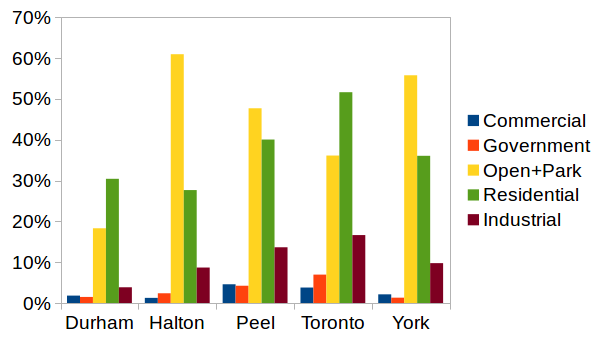
\includegraphics[width=0.7\textwidth]{media/area_use.png}};
%        \node[black] (B) at ($(A.south)!-.03!(A.north)$) {Region};
        \node[black,rotate=90] (C) at ($(A.west)!-.03!(A.east)$) {Percent of total land};
      \end{tikzpicture}
\caption{\label{fig:area_use}Distribution of region land uses.}
\end{figure}

The CHOICE survey includes data on home purchase price, or rent, but this does not give a clear picture of the overall market conditions and prices are given as of the year of purchase \cite{Papaioannou2014}. We supplement the survey data with real estate statistics compiled by the Toronto Real estate Board (TREB) \cite{TorontoRealEstateBoard2017}. They publish a monthly report outlining market prices aggregated to a custom set of 30 zones outside the City of Toronto and 36 zones within it. The TREB report classifies dwellings as detached, semi-detached, row/townhouse, condo townhouse, condo apartment, cooperative apartment, detached condo, and co-ownership apartment. We aggregate these classifications into house, townhouse, and condo for ease of analysis and to increase the sample size of each category. We further supplement these data with multiple listings service (MLS) records collected in May 2017 for both owned and rented dwellings. These data also include the area of each dwelling, number of bedrooms, and number of bathrooms. Figure ~\ref{fig:real_estate_price} provides annualized costs for each region and tenure type. For owned dwellings, a 25-year amortization period is employed, with an interest rate of 5\%, to obtain a representative annual cost \cite{RBC2018}. In the figure, each of the numbers (1,2,3) corresponds to a dwelling type (respectively: house, townhouse, and condo). It is evident that owned prices are significantly higher than rented prices; however, ownership gives the household possession of the asset and therefore includes an expected monetary return upon sale of the asset.

\begin{figure}[H]
\centering
        \begin{tikzpicture}
        \node[inner sep=0pt] (A) {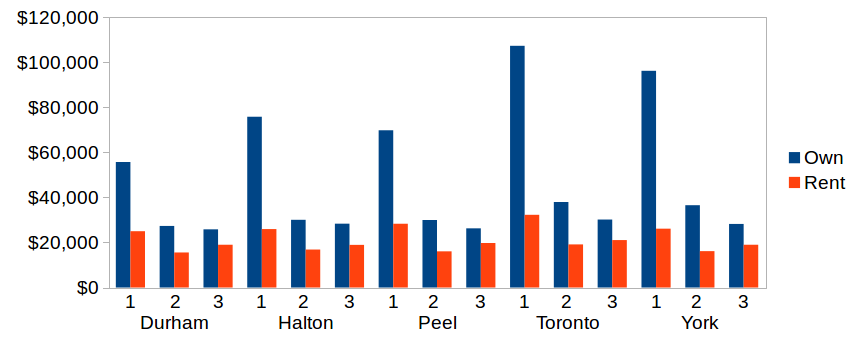
\includegraphics[width=\textwidth]{media/real_estate_price.png}};
%        \node[black] (B) at ($(A.south)!-.03!(A.north)$) {Region and Dwelling Type};
        \node[black,rotate=90] (C) at ($(A.west)!-.03!(A.east)$) {Annualized cost (\$)};
      \end{tikzpicture}
\caption{\label{fig:real_estate_price}Distribution of annualized cost by region and dwelling type.}
\end{figure}

\section{Model development}
The estimation of the bid-rent model requires multiple household agents to bid on each TAZ, with the winning agent being the one that is located in that TAZ. Using the RP data collected in the CHOICE survey, we only have the chosen location of each responding household and their characteristics. McFadden has proven that consistent parameter estimation can be performed using a random sample of alternative agents. Many previous studies of residential location choice use a smaller sample, but Nerella and Bhat provide a quantification of the error associated with smaller sampling rates \cite{Nerella2004}. Guided by their analysis, we take the household records from the CHOICE survey and associate them with 30 randomly selected households records from among those respondents who are not located in the same TAZ. We also explored a stratified importance sampling, taking 15 records from the same region and 15 from the same income group. However, this did not improve the significance of parameters or model goodness-of-fit. We define separate zones for each of the dwelling types considered in the model (i.e. house, townhouse, and condo), representing a simultaneous choice of zone and dwelling type by each household.

In most instances, unique explanatory variables can only be derived from the interaction of zone and household-specific attributes. A summary of the variables included in the final model is provided in Table ~\ref{tab:var_sum}. For example, the commuting drive time to work is a function of both the home and work location of a respondent. We assume that work locations are fixed, but the use of a record in the estimation of the expected bid in another TAZ requires an estimate of the commuting time from this unchosen home location. We, therefore, link the data with an inter-zonal matrix of AM peak auto commuting times from the GTA RTM. A second example of this interaction is the average dwelling area for each TAZ, which we interact with a household size of the respondent. Taking the natural logarithm of the household size provides a measure of dwelling area having a diminishing marginal influence on choice for each additional household member. In some instances, only the household attribute is used, as in the case of home to work distance. We divide this value by the income of each individual to obtain a measure of the sensitivity to commuting distance as a function of additional income. We assume this sensitivity to be a characteristic of the individual, independent of the TAZ they are considering - in contrast to the commuting time sensitivity, which is assumed fixed across respondents. The combination of these two variables accounts for the effect of proximity to the work location and differences between individuals arising from economic factors.

We define alternative-specific constants (ASC) by the membership of each household in an income quintile. This is similar to the models developed by Hurtubia in his original work \cite{Hurtubia2012}. In this initial exploration of the model, we define the individual utility weights by household role. Four roles are defined as follows: adult male, adult female, dependent child, and other member. It should be noted that there is some overlap between the characteristics of individuals holding an "adult" or "child" role in the dataset. The "child" role generally refers to individuals under the age of 18, but may include older individuals who still live with their parents (e.g. university students). This distinction is deemed valid as the weights denote the role each individual plays in determining the residential location choice. In the case of an individual, over the age of 18 and living at home, it is likely they were younger at the time of the residential location choice. In contrast, the same individual likely had a greater influence on the decision if they are listed as an "adult" and they are the owner of the dwelling. This partially explains the result in Table ~\ref{tab:data_sum}. The average commuting time for those given the role "child" is similar to, or higher than, the "adult" roles for most regions. There are two households with individuals listed as "child" who are aged 35 to 44. With the caveat that the sample size makes this largely anecdotal, the mean commuting time for these individuals is 47 minutes, which is well above the regional average.

\begin{longtable}{l r l}
\caption{Development of model variables.}
  \label{tab:var_sum}\\
  \toprule
Variable &    TAZ property $\times$ &  HH property \\
\midrule
\endfirsthead
\caption[]{(continued)}\\
\toprule
Variable &    TAZ property $\times$ &  HH property \\
\midrule
\endhead
\multicolumn{3}{c}{\textbf{Individual Variables}} \\
HW distance & & \makecell[l]{Home to work commute\\distance / individual income} \\
HW auto time & \makecell[r]{Inter-zonal home-to-work\\auto travel time (min.)} & Exogenous work TAZ \\
Park cost & & \makecell[l]{Cost of parking at work\\location (10s \$ per month)} \\
Transit & \makecell[r]{Count of GO Train stations within\\3 km or TTC stations within 500 m\\of zone centroid} & \makecell[l]{Individual has transit\\pass (0/1)} \\
\makecell[l]{Frequency\\auto} & & \makecell[l]{Frequency of individual\\commute by auto} \\
HW TAZ & \makecell[r]{Home and work location\\in same TAZ (0/1)} & Exogenous work TAZ  \\
\multicolumn{3}{c}{\textbf{Household Variables}} \\
House & House (0/1) & 2+ HH members (0/1) \\
High income & \makecell[r]{Mean HH income in top\\income quintile (0/1)} & \makecell[l]{HH income in top\\income quintile (0/1)}  \\
Low income & \makecell[r]{Mean HH income in top\\income quintile (0/1)} & \makecell[l]{HH income in bottom\\income quintile (0/1)}  \\
Dwelling area & \makecell[r]{Average dwelling\\area (100s $m^2$)} & ln(HH size)  \\
Veh/lic & & HH vehicles / HH licenses  \\
Children & & Number of children in HH  \\
INC\_2 & & HH income in 2nd quintile \\
INC\_3 & & HH income in 3rd quintile \\
INC\_4 & & HH income in 4th quintile \\
INC\_5 & & HH income in top quintile \\
\multicolumn{3}{c}{\textbf{Weights}} \\
W\_Role1 & & Adult male \\
W\_Role2 & & Adult female \\
W\_Role3 & & Dependent child \\
W\_Role4 & & Other member \\
W\_Age & & Age of HH member \\
\bottomrule
\end{longtable}

\section{Model Estimation Results}
The results of the estimation are outlined in Table ~\ref{tab:model_sum} for the final model. A wide variety of intermediate models were estimated, including standard bid-rent models (excluding the latent auction component) for each model. The majority of the parameters are significant (at the 0.05 level of significance) and have intuitive signs. Critically, home to work auto travel time has a negative parameter and dwelling area is found to have a positive parameter, both being significant. The house variable - representing the probability of a household with 2, or more, members choosing a house dwelling type - has a negative sign. Looking at the corresponding bid-rent function, the sign is consistently positive in models that include this variable. Hurtubia \emph{et al.} obtain a similar result for this variable \cite{Hurtubia2017}, which are concentrated in more outlying areas of the GTA. These outlying areas are characterized by lower dwelling prices, relative to those in the City of Toronto proper. The negative sign on the parameter suggests that larger households, who have higher living expenses, value the lower priced houses located in the outlying suburbs.

We find a common parameter value for locating proximate to TTC stations and GO Train stations, given the bounding radii defined for each station type. This suggests that households tend to \emph{ceteris paribus} value being located within 500 m of a TTC station in a similar way to being located within 3 km of a GO Train station. A negative sign is obtained for the number of vehicles per licensed driver, which suggests that households tend to trade-off a higher priced dwelling against the ownership of additional vehicles. This is consistent with other parameter values in that transit proximity is positively valued and larger households tend to locate in outlying areas, with poor transit service, requiring the purchase of additional vehicles.

With respect to individual weights, weights are estimated in the final model for four household roles (i.e. adult male, adult female, dependent child, and other). A challenge in estimating these weights is the requirement for a reference weight in the MNL weight function, against which to measure the relative utility for other household members. Household compositions in the sample are not uniform, such that a single role cannot be fixed as the reference. For example, a household may contain two adult males or no adult males. We reference the weight of each household member against the role of the responding member. It is interesting to note that this model does not suggest a strong difference in the weight of male and female influence on residential location choice - in contrast to prior studies on the subject \cite{Chiappori2014, Picard2013}. In a household with a single male/female couple, the weights are 0.49 and 0.51, respectively. Given the aforementioned caveats about the overlap between "adult" and "child" roles, we included a weighting variable for the age of the household member. Although not strongly significant, this suggests that age plays a strong role in the weight of the individual on residential location choice. We explored the inclusion of several other variables, including individual work status and income, but the sample data is incomplete for these variables and their inclusion did not have a significant effect on the model.

\begin{longtable}{lrrr}
\caption{Model parameter statistics.}
\label{tab:model_sum} \\
\toprule
Variable &    Value &  Std err. &    t-stat \\
\midrule
\endfirsthead
\caption[]{(continued)}\\
\toprule
Variable &    Value &  Std err. &    t-stat \\
\midrule
\endhead
\multicolumn{4}{c}{\textbf{Individual Variables}} \\
HW auto travel time & -0.03 & 0.003 & -11.84 \\
Parking cost at school or work & 0.02 & 0.006 & 2.45 \\
Transit & 0.35 & 0.12 & 2.99 \\
Frequency auto & 1.99 & 0.17 & 11.43 \\
HW TAZ & 0.63 & 0.10 & 6.27 \\
\multicolumn{4}{c}{\textbf{Household variables}} \\
House & -0.31 & 0.02 & -14.29 \\
High income & 0.28 & 0.10 & -3.04 \\
Low income & -0.25 & 0.21 & -1.16 \\
HW distance & 1.16 & 0.24 & 4.87 \\
Dwelling area & 0.26 & 0.04 & 6.20 \\
Veh/lic & -0.52 & 0.08 & -6.58 \\
Children & -0.15 & 0.05 & -3.01  \\
INC\_2 & 0.08 & 0.27 & 0.32 \\
INC\_3 & 0.36 & 0.19 & 1.91 \\
INC\_4 & 0.38 & 0.20 & 1.90 \\
INC\_5 & 0.37 & 0.19 & 1.96 \\
\multicolumn{4}{c}{\textbf{Weights}} \\
W\_Role1 & -0.93 & 0.53 & -2.39 \\
W\_Role2 & -0.87 & 0.64 & -2.24 \\
W\_Role3 & -1.18 & 0.64 & -3.24 \\
W\_Role4 & -0.74 & 0.46 & -2.63 \\
W\_Age & -0.12 & 0.28 & -1.10 \\
\multicolumn{4}{c}{\textbf{Price variables}} \\
$\gamma$ & 0.41 & 0.04 & 9.73 \\
$\alpha$ & 9.17 & 0.21 & 43.04 \\
$\sigma$ & 0.25 & 0.006 & 39.49 \\
$\rho^2$ (const) & 0.04 & & \\ 
$\rho^2$ (null) & 0.04 & & \\ %(Hurtubia gets just under 0.10 in thesis using larger dataset.
\bottomrule
\end{longtable}

Another avenue of exploration was considering variation in household composition by distinguishing the adult role weights based on whether the household includes children. This would account for differences in the role of an adult by their consideration for school location and altruism for their children. However, no significant difference was found between these variables. This effect is partially considered through the inclusion of the age weight and variable in the household utility function indicating whether the household includes children (under the age of 13). A series of other weight configurations were explored for adult roles including: separate weights for single and multi-worker household adults, separate weights for single and multi-member household adults, and the addition of a weight for full-time work status. We also considered models wherein the individual utilities were separated into weighted and unweighted components. None of these changes significantly improved the model fit or provided statistical insights into intra-household dynamics.

\subsection{Elasticity analysis}
A robust and tangible method of examining the magnitude of parameter values is obtained from calculation of the elasticities with respect to each explanatory variable. In the case of continuous variables, this takes the form of a point elasticity, while category variables require the use of an arc elasticity measured between variable states. We present a combined plot for a subset of continuous variables in Figure ~\ref{fig:elasticity}. It is evident that there is a large positive elasticity between the probability of a household choosing to locate in a TAZ and the average dwelling area for that TAZ-dwelling type pair. A graphical representation helps to draw out the similarity in elasticities between the adult male/female roles with respect to their sensitivity to auto travel time and parking cost at school or work. It is also clear that the influence of dependent children on residential location choice is weaker.

\begin{figure}[H]
\centering
        \begin{tikzpicture}
        \node[inner sep=0pt] (A) {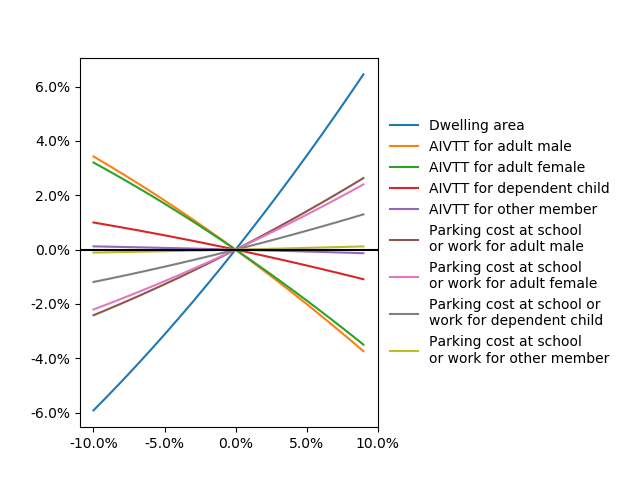
\includegraphics[width=1.0\textwidth]{media/elasticity.png}};
        \node[black] (B) at (-1.75,-5) {\% change in variable value};
        \node[black,rotate=90, align=center] (C) at ($(A.west)!-.02!(A.east)$){\% change in probability\\of HH being located in TAZ};
      \end{tikzpicture}
\caption{\label{fig:elasticity}Elasticities for representative variables.}
\end{figure}

\section{Discussion of Model Results}

\section{Chapter Conclusions}
This paper adds to the growing literature on intra-household dynamics in residential location choice. By considering such dynamics, we can better capture the decision-making process and consider a wider range of policy scenarios. We provide an independent confirmation of the bid-auction approach recently proposed by Hurtubia \emph{et al.} \cite{Hurtubia2017}. The present analysis suggests a weakening differential in the influence of male and female household members on residential location choice. This fits with a continued shift towards higher labour force engagement, whereby the household must consider the work location of several members. We find that larger households remain constrained in their ability to locate in urban areas, proximate to their work location. Whether this is an outcome of high land prices or a lack of available housing stock, single-family houses continue to be the domain of outlying suburban areas, with low land prices and high automobile dependence.

This study presents a strong basis for further research. However, it could be improved through the collection of a sample that includes households who work within the same city. A major bias, existing in most residential location choice models, is the so-called modifiable areal unit problem (MAUP). This arises from the use of arbitrary aggregations of spatial units, a standard practice in residential location choice models. We explored the inclusion of a spatial lag term in our model to account for this bias. Lags were considered for the co-location of similar income households, similar sized households, and by tenure (i.e. own or rent dwelling). Results are preliminary, but this direction holds promise for additional insights with respect to household dynamics and social factors.
\chapter{Household Production Function}
\section{Introduction}

\section{Model Formulation}

\section{Data Description}

\section{Model Estimation Results}

\section{Discussion of Model Results}

\section{Chapter Conclusions}
\chapter{AV and Residential Location Choice}
\section{Introduction}

\section{Model Formulation}

\section{Data Description}

\section{Model Estimation Results}

\section{Discussion of Model Results}

\section{Chapter Conclusions}
\chapter{TBD}
\chapter{Conclusions and Future Work}

%% This adds a line for the Bibliography in the Table of Contents.
\addcontentsline{toc}{chapter}{Bibliography}
%% *** Set the bibliography style. ***
%% (change according to your preference/requirements)
\bibliographystyle{plain}
%% *** Set the bibliography file. ***
%% ("thesis.bib" by default; change as needed)
\bibliography{thesis}

%% *** NOTE ***
%% If you don't use bibliography files, comment out the previous line
%% and use \begin{thebibliography}...\end{thebibliography}.  (In that
%% case, you should probably put the bibliography in a separate file and
%% `\include' or `\input' it here).

\end{document}
